\documentclass{beamer}

\title{The Kanban Method}
\begin{document}
    
\begin{frame}

    \maketitle

\end{frame}
\begin{frame}
    \begin{itemize}
        \item 'Kanban' is a Japanese word meaning billboard \textbackslash signboard. 
        \item The kanban method comes from the car industry in Japan.
        \item This method was invented in the late 40's, by Toyota.
        \item The goal was to optimize the car production and be more competitive with American companies.
        \item The main idea is to be able to produce on demand, "just in time".
        \item The software industry began to use it at the beginning of the 21st Century.
        \item It helps you visualize your work and maximize your efficiency.
    \end{itemize}  

\end{frame}
\begin{frame}{The Concept}
    \begin{itemize}
        \item a non-disruptive evolutionary change management system
        \item implementing many minor changes rather than a large one
        \item visualising the workflow
    \end{itemize}
     \begin{figure}
      \centering
   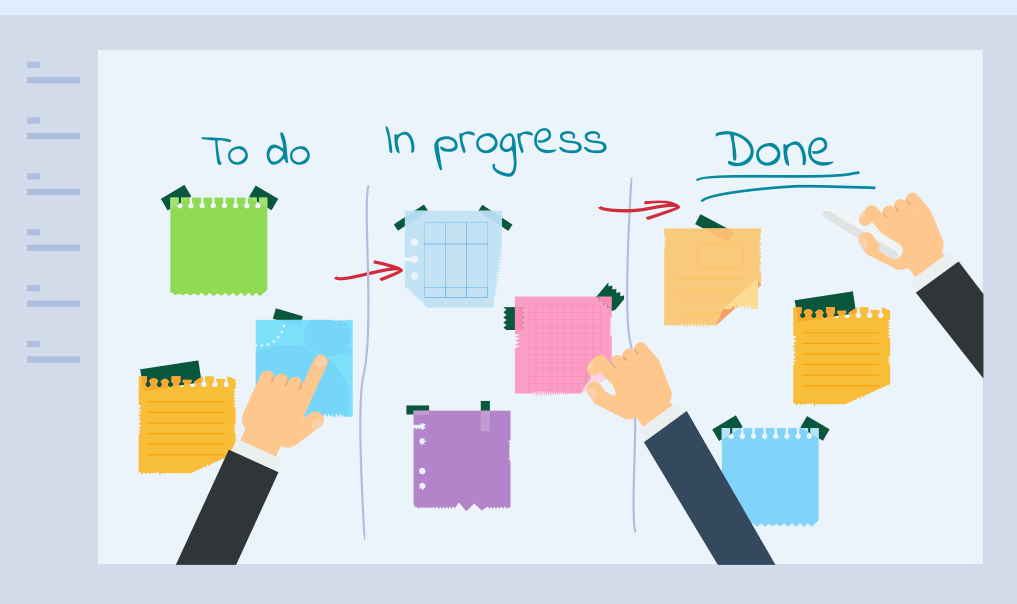
\includegraphics[scale=0.5]{ph.png}
      \caption{Task's board}
    \end{frame}
\end{document}

\end{frame}
\begin{frame}{Advantages}
    \begin{itemize}
        \item avoid waste
        \item do on-demand production
        \item reduction of production costs
        \item quick to set up this method and not expensive
        \item more flexibility in the production
    \end{itemize}
